\scanpage{22}
$\mathcal E^{2n}$ \deleted{is generated by} \inserted{admits the \uline{basis}} $L_0^n$,
\inserted{(for a fixed Lefschetz $L_0$)}
\deleted{$\mathcal E^{-2n}$ \unsure{generated} by $\Lambda_0^n$,}
\deleted{for a choice of $(L,\Lambda)$.}
\deleted{of $\mathcal E^{2n}$, \illegible{2} of $L'$.}
Now.\,--- where, if $L'$ is another Lefschetz element
\figure{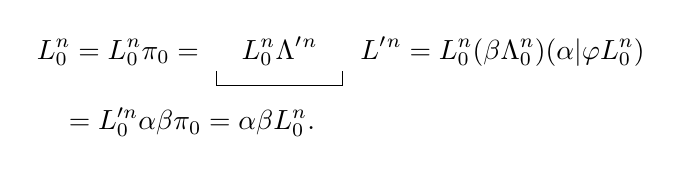
\begin{tikzpicture}
\node[anchor=base east] at(-.9,0){$\displaystyle L_0^n=L_0^n\pi_0=$};
\node[anchor=base] at(0,0){$\displaystyle L_0^n\Lambda'{}^n$};
\node[anchor=base west] at(.9,0){$\displaystyle L'{}^n=L_0^n(\beta\Lambda_0^n)(\unsure{\alpha|\varphi}L_0^n)$};
\draw(-.8,-.15)--(-.8,-.33)--(.8,-.33)--(.8,-.15);
\node[anchor=base west] at(-2.8,-.9){$\displaystyle =L_0^{\prime n}\alpha\beta\pi_0=\alpha\beta L_0^n.$};
\end{tikzpicture}}
which proves that $\alpha\beta=1$, hence $\alpha$ and $\beta$ invertible, hence \deleted{\unsure{for}} $\unsure{L_0^{\prime n}|L_0^n|L'{}^n}$ and $\unsure{\Lambda_0^{\prime n}|\Lambda_0^n|\Lambda'{}^n}$ are bases of $\mathcal E^{(2n)}$ and $\mathcal E^{(-2n)}$ respectively.

Whence
\diagram{\begin{tikzcd}[ampersand replacement=\&,column sep=large]
L^{\unsure{\prime|*}}\ \text{Lefschetz}\arrow[r,Rightarrow]\&L^n\ \text{\uline{a basis of}}\ \mathcal E^{2n}
\end{tikzcd}}
\figure{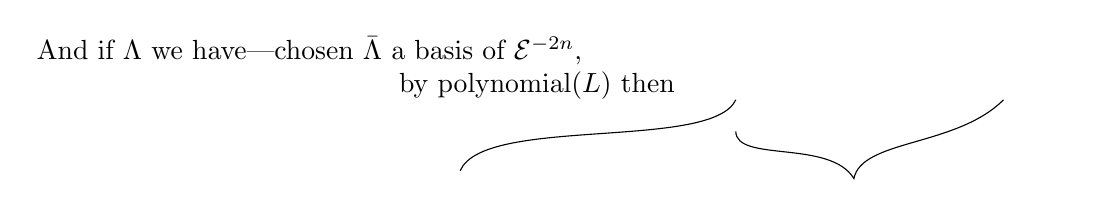
\begin{tikzpicture}[x=1cm,y=1cm]
\node[anchor=west,align=left,text width=13cm] at (0,1.1) {\inserted{And if $\deleted{\unsure{\Lambda}}$ \unsure{we have|chosen} $\bar\Lambda$ a basis of $\mathcal E^{-2n}$,\\\hspace*{4.6cm}by \uline{\unsure{polynomial}}$(L)$ then}};
\draw (5.5,-.2) .. controls (5.8,.5) and (8.7,.05) .. (9,.7);
\draw (9,.3) .. controls (9,-.1) and (10.2,.2) .. (10.5,-.3) .. controls (10.6,.2) and (11.8,.1) .. (12.4,.7);
\end{tikzpicture}}
\margin{?}
We know how to prove a converse, in the case where \deleted{$\unsure{\mathcal E}$} $\mathcal E$ is finitely generated projective over $k$. This certainly does not work as it stands, for example for $\mathcal E=\mathcal L(M^*)$, $M^*$ graded in degrees $0\leq i\leq4$ ---.

But this does not work either for the endomorphisms associated with the elements of degree $2$ of a Lefschetz algebra, for dimension $6$

$\mathcal E$ generated by $L,L'$ \inserted{\figure{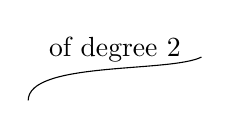
\begin{tikzpicture}
\node at(0,0){of degree $2$};
\draw(-1.1,-.65) .. controls(-1.1,-.15) and(.7,-.3) .. (1.1,-.1);
\end{tikzpicture}}} with the relations
\[
L^4=0,\quad L'^2-LL'=0,\quad L^2L'-L^3=0,\quad L^3L'=0,\qquad\text{with basis}
\]
\diagram{\begin{array}{r c||c||c||c}
&1&L,L'&L^2,LL'&L^3\\\cline{2-5}
\text{degree:}&0&2&4&
\end{array}}
\margin{\figure{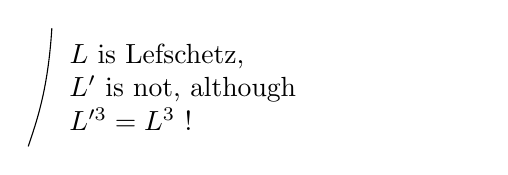
\begin{tikzpicture}
\draw(.3,1.5) .. controls(.25,.7) and(.1,.3) .. (0,0);
\node[anchor=west,align=left,text width=5.1cm] at(.4,.75){$L$ is Lefschetz,\\$L'$ is not, although\\$L'^3=L^3$ !};
\end{tikzpicture}}}
\mspage{21}
